\section{习题一 \ Runge现象}


1. 下段代码即为Lagrange插值法计算函数。\inputpython{E:/numerical-approximation/code/project2_1.py}{21}{32}
2. 用下段代码生成等距节点。然后代入上述第一问Lagrange函数进行计算即可。\inputpython{E:/numerical-approximation/code/project2_1.py}{36}{39}

\begin{figure}[htbp]
    \centering
    \subfigure[$n=4$]
    {
        \begin{minipage}[b]{.4\linewidth}
            \centering
            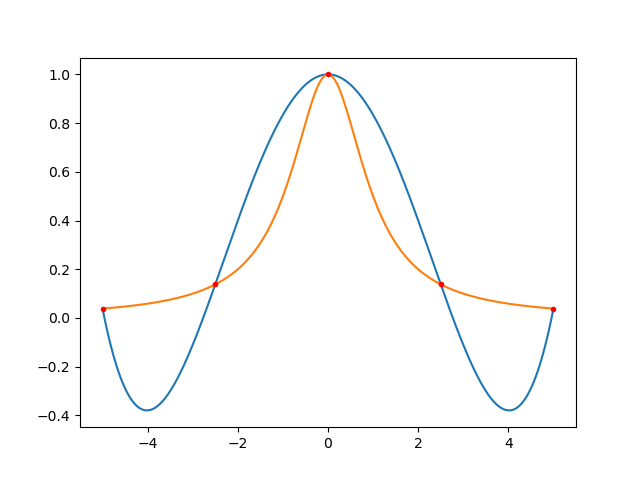
\includegraphics[scale=0.29]{pic/n=4.png}
        \end{minipage}
    }
    \subfigure[$n=10$]
    {
        \begin{minipage}[b]{.4\linewidth}
            \centering
            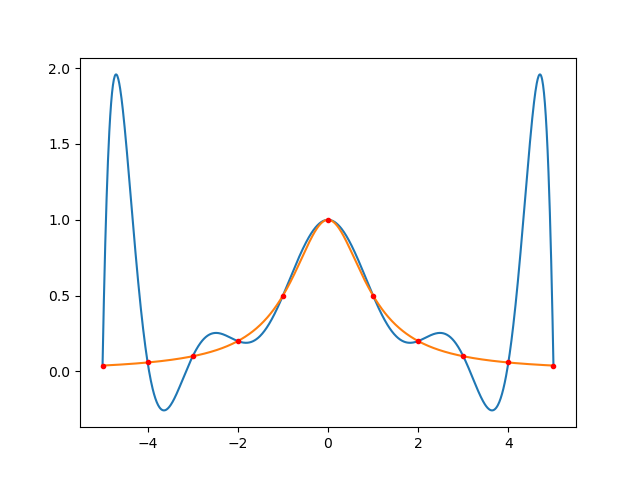
\includegraphics[scale=0.29]{pic/n=10.png}
        \end{minipage}
    }
    \subfigure[$n=14$]
    {
        \begin{minipage}[b]{.4\linewidth}
            \centering
            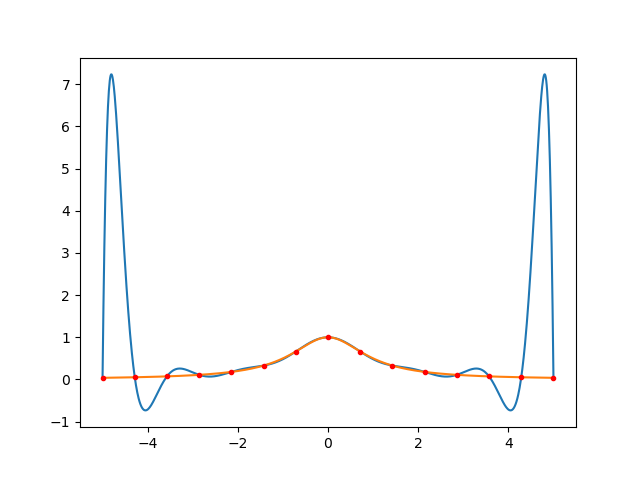
\includegraphics[scale=0.29]{pic/n=14.png}
        \end{minipage}
    }
    \subfigure[$n=20$]
    {
        \begin{minipage}[b]{.4\linewidth}
            \centering
            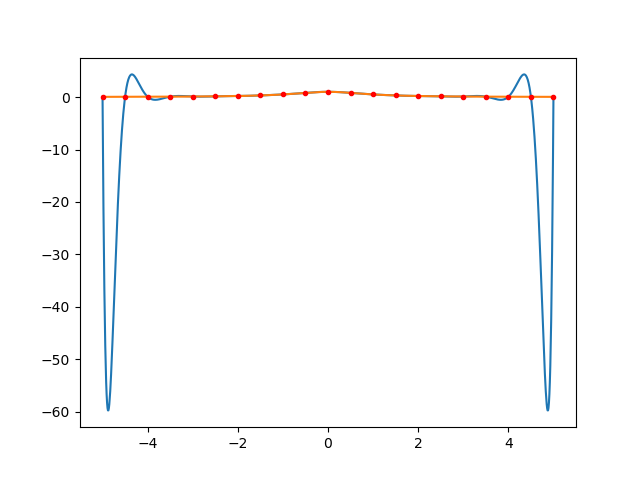
\includegraphics[scale=0.29]{pic/n=20.png}
        \end{minipage}
    }
    \caption{等距节点差值}
\end{figure}
3. 用下段函数构造chebyshev节点。然后再带入第一问Lagrange函数计算即可。\inputpython{E:/numerical-approximation/code/project2_1.py}{44}{47}
\begin{figure}[htbp]
    \centering
    \subfigure[$n=4$]
    {
        \begin{minipage}[b]{.4\linewidth}
            \centering
            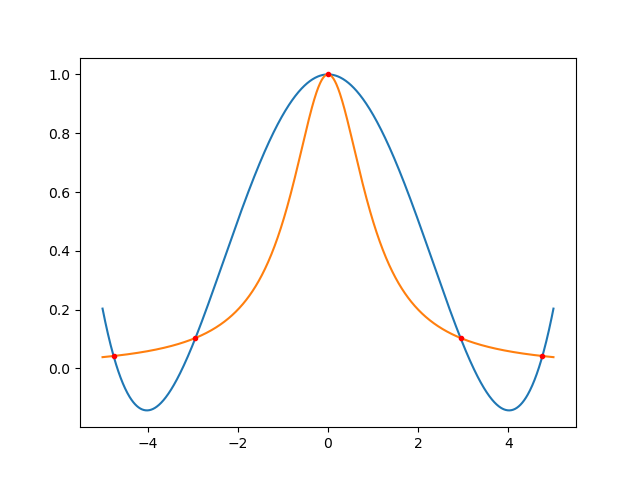
\includegraphics[scale=0.29]{pic/chebyshev/4.png}
        \end{minipage}
    }
    \subfigure[$n=10$]
    {
        \begin{minipage}[b]{.4\linewidth}
            \centering
            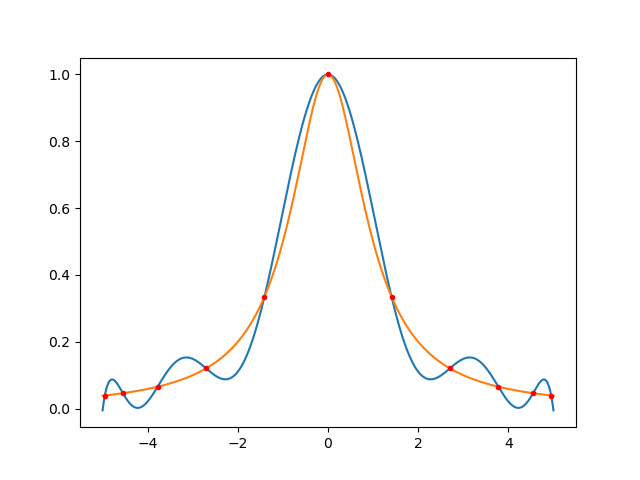
\includegraphics[scale=0.29]{pic/chebyshev/10.png}
        \end{minipage}
    }
    \subfigure[$n=14$]
    {
        \begin{minipage}[b]{.4\linewidth}
            \centering
            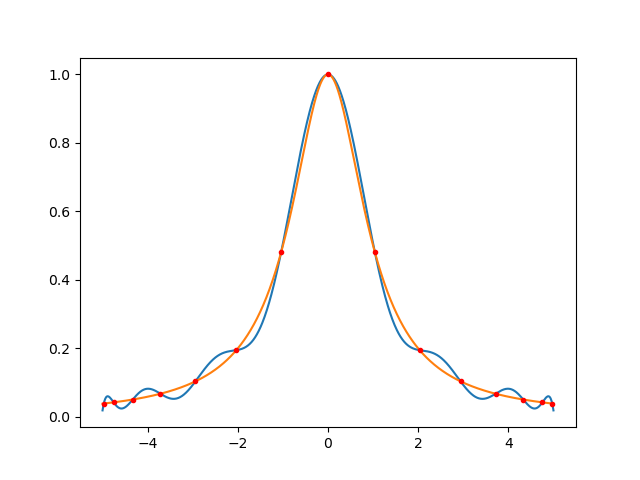
\includegraphics[scale=0.29]{pic/chebyshev/14.png}
        \end{minipage}
    }
    \subfigure[$n=20$]
    {
        \begin{minipage}[b]{.4\linewidth}
            \centering
            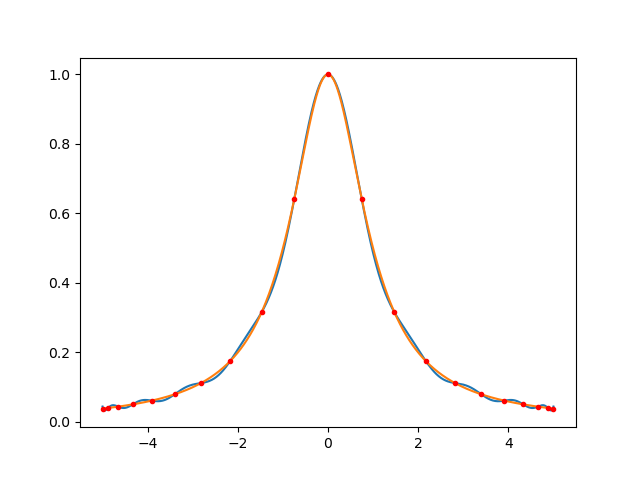
\includegraphics[scale=0.29]{pic/chebyshev/20.png}
        \end{minipage}
    }
    \caption{chebyshev节点差值}
\end{figure}
4.Newton插值法
\begin{figure}[htbp]
    \centering

    {
        \begin{minipage}[b]{.9\linewidth}
            \centering
            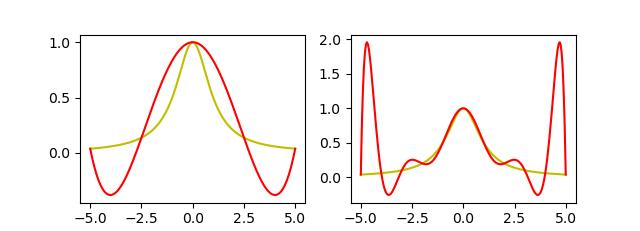
\includegraphics[scale=0.6]{pic/newton(1).png}
        \end{minipage}
    }


\end{figure}
\begin{figure}[htbp]
    \centering

    {
        \begin{minipage}[b]{.9\linewidth}
            \centering
            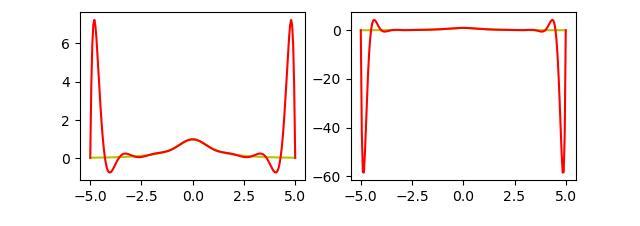
\includegraphics[scale=0.6]{pic/newton(2).png}
        \end{minipage}
    }


    \caption{chebyshev节点差值}
\end{figure}
\section{习题二 \ 分段差值}
1.分段线性插值方法
\begin{figure}[htbp]
    \centering

    {
        \begin{minipage}[b]{.9\linewidth}
            \centering
            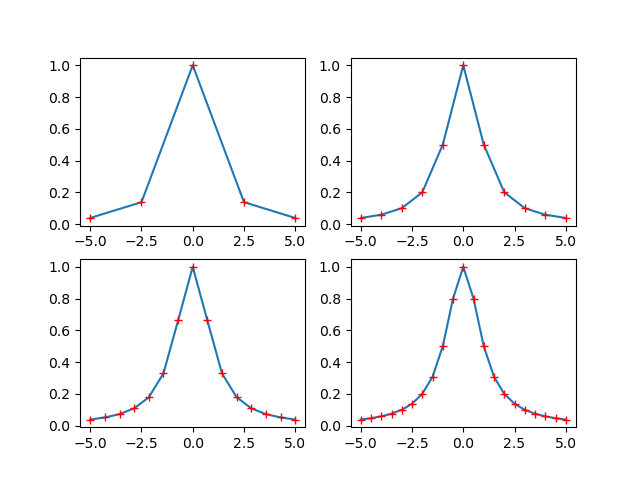
\includegraphics[scale=0.6]{pic/线性插值.png}
        \end{minipage}
    }


    \caption{分段线性插值方法}
\end{figure}

2.分段3次Hermite插值方法
\begin{figure}[htbp]
    \centering
    \subfigure[$n=4$]
    {
        \begin{minipage}[b]{.4\linewidth}
            \centering
            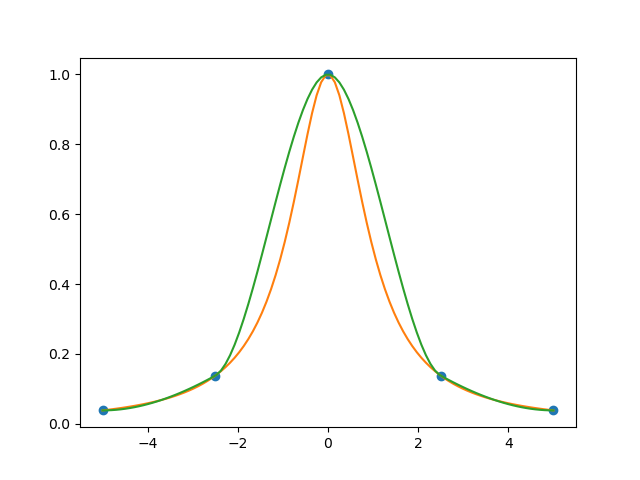
\includegraphics[scale=0.29]{pic/hermit/4.png}
        \end{minipage}
    }
    \subfigure[$n=10$]
    {
        \begin{minipage}[b]{.4\linewidth}
            \centering
            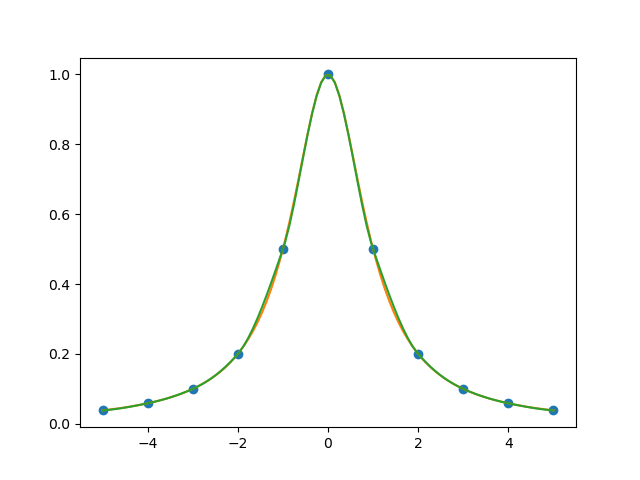
\includegraphics[scale=0.29]{pic/hermit/10.png}
        \end{minipage}
    }
    \subfigure[$n=14$]
    {
        \begin{minipage}[b]{.4\linewidth}
            \centering
            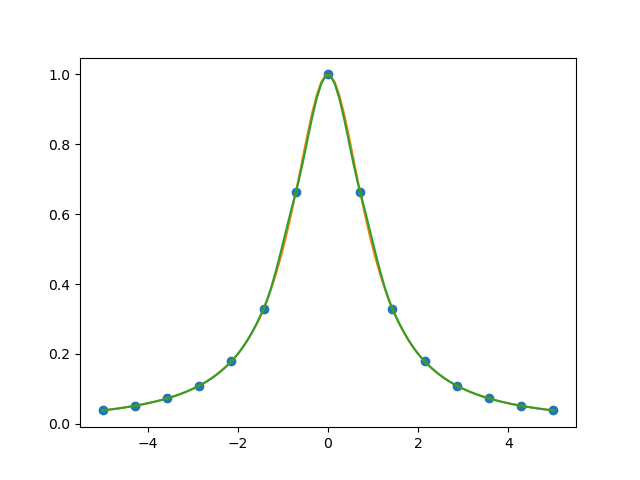
\includegraphics[scale=0.29]{pic/hermit/14.png}
        \end{minipage}
    }
    \subfigure[$n=20$]
    {
        \begin{minipage}[b]{.4\linewidth}
            \centering
            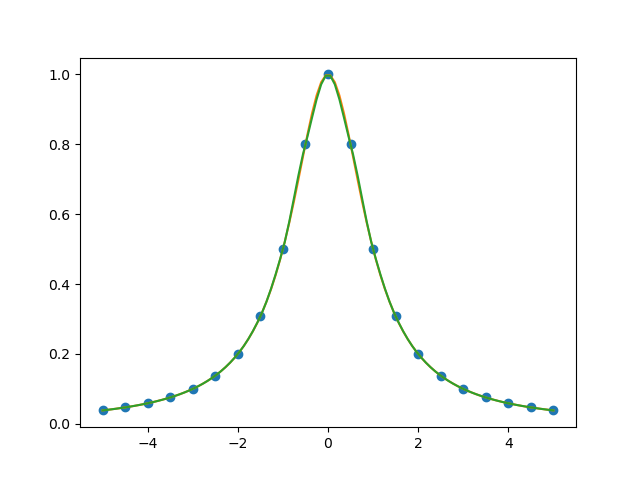
\includegraphics[scale=0.29]{pic/hermit/20.png}
        \end{minipage}
    }
    \caption{分段3次Hermite插值方法}
\end{figure}
\clearpage
3.三次样条插值方法
\begin{figure}[htbp]
    \centering
    \subfigure[$n=4$]
    {
        \begin{minipage}[b]{.4\linewidth}
            \centering
            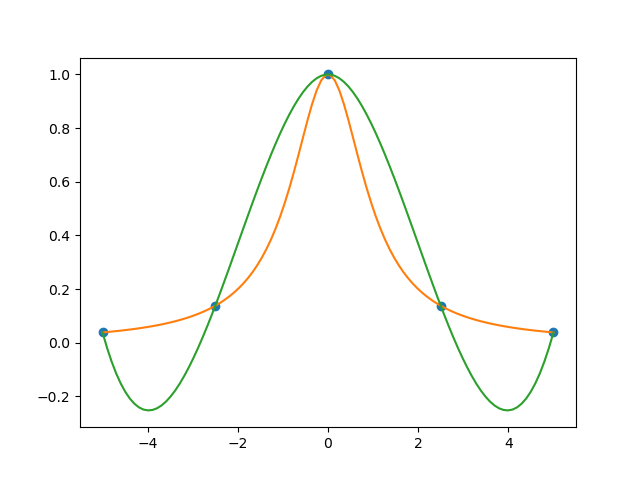
\includegraphics[scale=0.29]{pic/三次样条/4.png}
        \end{minipage}
    }
    \subfigure[$n=10$]
    {
        \begin{minipage}[b]{.4\linewidth}
            \centering
            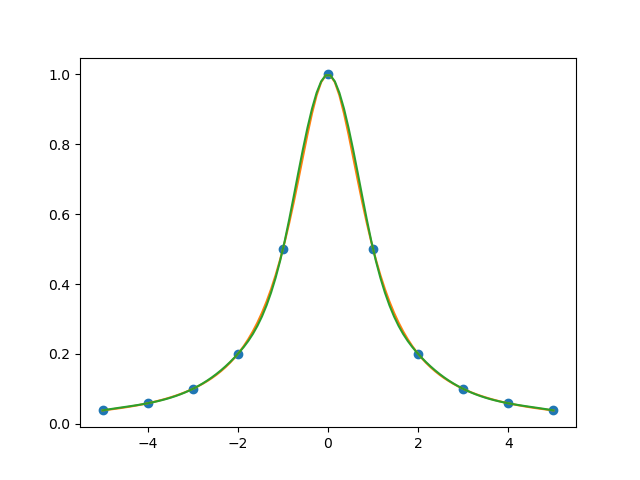
\includegraphics[scale=0.29]{pic/三次样条/10.png}
        \end{minipage}
    }
    \subfigure[$n=14$]
    {
        \begin{minipage}[b]{.4\linewidth}
            \centering
            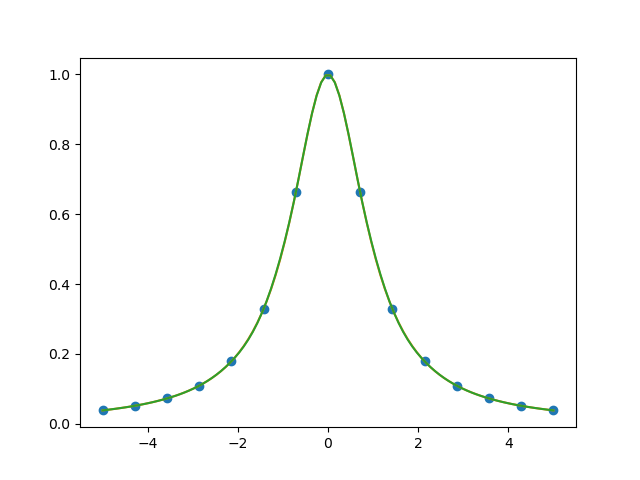
\includegraphics[scale=0.29]{pic/三次样条/14.png}
        \end{minipage}
    }
    \subfigure[$n=20$]
    {
        \begin{minipage}[b]{.4\linewidth}
            \centering
            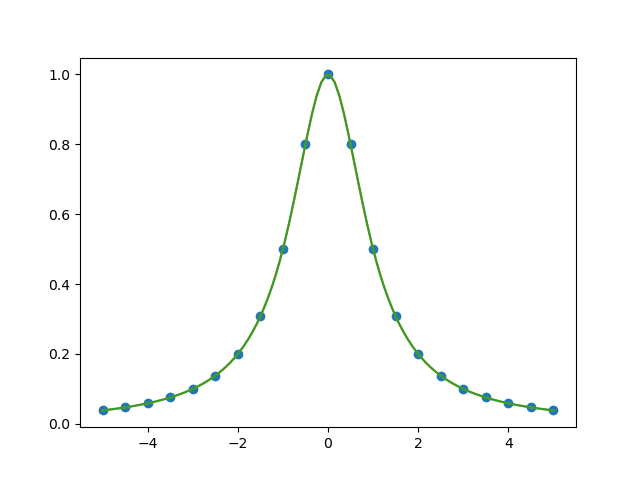
\includegraphics[scale=0.29]{pic/三次样条/20.png}
        \end{minipage}
    }
    \caption{三次样条插值方法}
\end{figure}

\section{习题三 \ 物体轨迹}

\begin{figure}[htb]
    \centering

    {
        \begin{minipage}[b]{.9\linewidth}
            \centering
            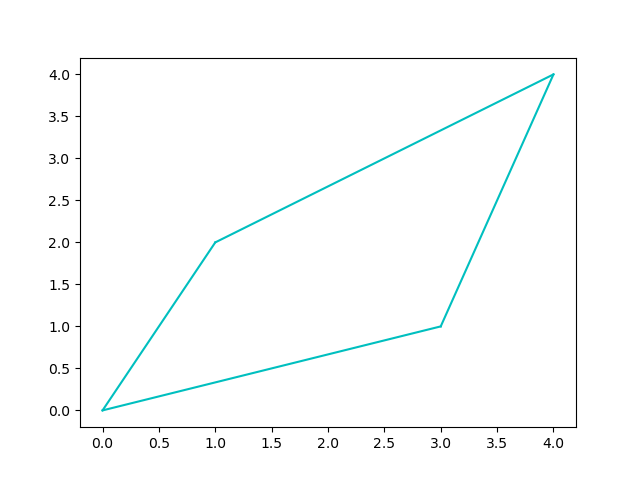
\includegraphics[scale=0.6]{pic/物体轨迹/linear2.png}
        \end{minipage}
    }


    \caption{分段线性插值方法}
\end{figure}

\begin{figure}[htb]
    \centering

    {
        \begin{minipage}[b]{.9\linewidth}
            \centering
            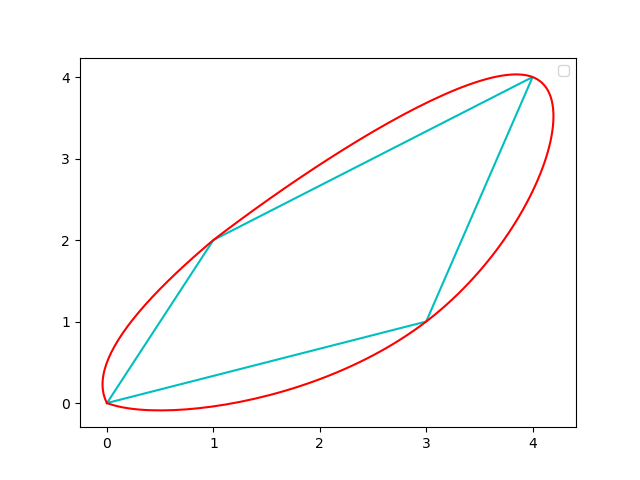
\includegraphics[scale=0.6]{pic/物体轨迹/cubic2.png}
        \end{minipage}
    }


    \caption{三次样条插值方法}
\end{figure}